\section{Parallelverarbeitung}\label{sec:parallelverarbeitung}

\subsection{Parallele Bearbeitung einer Aufgabe}

\begin{defi}{Parallelverarbeitung}
    % TODO: https://de.wikipedia.org/wiki/Nebenl%C3%A4ufigkeit (Quelle)
    Die \emph{Parallelverarbeitung} (engl. \enquote{concurrency}), zielt darauf ab, mehrere Aufgaben, Berechnungen, Anweisungen oder Befehle gleichzeitig ausführen zu können.
    Es kann sich dabei um völlig unabhängige Anweisungen handeln, bis hin zur gemeinsamen Bearbeitung einer Aufgabe.
    
    Ziel ist eine \emph{Leistungssteigerung}.
    
    Voraussetzungen sind, dass
    \begin{itemize}
        \item eine Aufteilungsmöglichkeit existiert und erkannt wird,
        \item mehrere Bearbeiter zur Verfügung stehen und
        \item diese gleichzeitig und dabei möglichst unabhängig agieren können.
    \end{itemize}
\end{defi}

\begin{defi}{Domain Decomposition}
    \emph{Domain Decomposition} bzw. \emph{Gebietszerlegung} beschreibt die statische oder dynamische Aufteilung eines Datengebiets in Bereiche gleicher Prozessorarbeit.
    Alle Gebiete werden mit demselben Programmteil parallel verarbeitet.
    
    Domain Decomposition ist insbesondere geeignet für \emph{homogene Plattformen}.
    
    Im High-Performance-Computing (HPC) wird diese Art der Parallelisierung häufigsten verwendet.
\end{defi}

\begin{defi}[Domain Decomposition]{Statische Aufteilung}
    % TODO: https://de.wikipedia.org/wiki/Lastverteilung_(Informatik) (Quelle)
    \emph{Statische Aufteilung} der Domain Decomposition berücksichtigt den Zustand verschiedener Maschinen nicht.
    Sie soll z. B. die Kommunikation zwischen Prozessoren minimieren, oder bestimmte Hardware-Eigenschaften des Verbindungsnetzwerkes ausnutzen.
    
    Der Vorteil statischer Aufteilung ist, dass sie leicht zu implementieren und bei relativ regelmäßigen Aufgaben äußerst effizient ist.
\end{defi}

\begin{example}[Domain Decomposition]{Statische Aufteilung}
    TODO: Grafik
\end{example}

\begin{defi}[Domain Decomposition]{Dynamische Aufteilung}
    % TODO: https://de.wikipedia.org/wiki/Lastverteilung_(Informatik) (Quelle)
    \emph{Dynamische Aufteilung} der Domain Decomposition soll ein Gebiet in Bereiche gleicher Prozessorarbeit aufteilen.
    
    Im Gegensatz zur statischen Aufteilung wird bei der dynamische Variante die aktuelle Last jeder der Recheneinheiten im System berücksichtigt.
    Bei diesem Ansatz können Aufgaben dynamisch von einem überlasteten Knoten zu einem unterlasteten Knoten verschoben werden, um eine schnellere Verarbeitung zu erhalten.
    
    Obwohl diese Algorithmen viel komplizierter zu entwerfen sind, können sie hervorragende Ergebnisse liefern, insbesondere wenn die Ausführungszeit von einer Aufgabe zur anderen stark variiert.
    
\end{defi}

\begin{example}[Domain Decomposition]{Dynamische Aufteilung}
    TODO: Grafik
\end{example}

\begin{defi}{Functional Decomposition}
    \emph{Functional Decomposition} bzw. \emph{Funktionsaufteilung} beschreibt die Zerlegung eines Problems in unterschiedliche Programmteile, Unterprogramme oder Module, die dann auf Prozessoren verteilt und parallel bearbeitet werden.
    
    Dabei können die Programmteile auf jeweils unterschiedlichen, eventuell spezialisierten, Rechnerarchitekturen ausgeführt werden.
\end{defi}

\begin{jsc}[Functional Decomposition]{Modulare Supercomputing Architektur}
    % TODO: https://www.fz-juelich.de/de/ias/jsc/ueber-uns/struktur/forschungsgruppen/jsc-rg-proto/modulare-supercomputing-architektur (Quelle)
    Die \emph{Modular Supercomputing Architecture} (\emph{MSA}) ist ein Systemdesign zur Integration heterogener Ressourcen und zur Erfüllung der Anforderungen eines breiten Spektrums von Anwendungsbereichen, die von rechenintensiven, hochskalierenden Simulationscodes bis hin zu datenintensiven Workflows der künstlichen Intelligenz reichen.
    
    \vspace{1em}
    
    \centering
    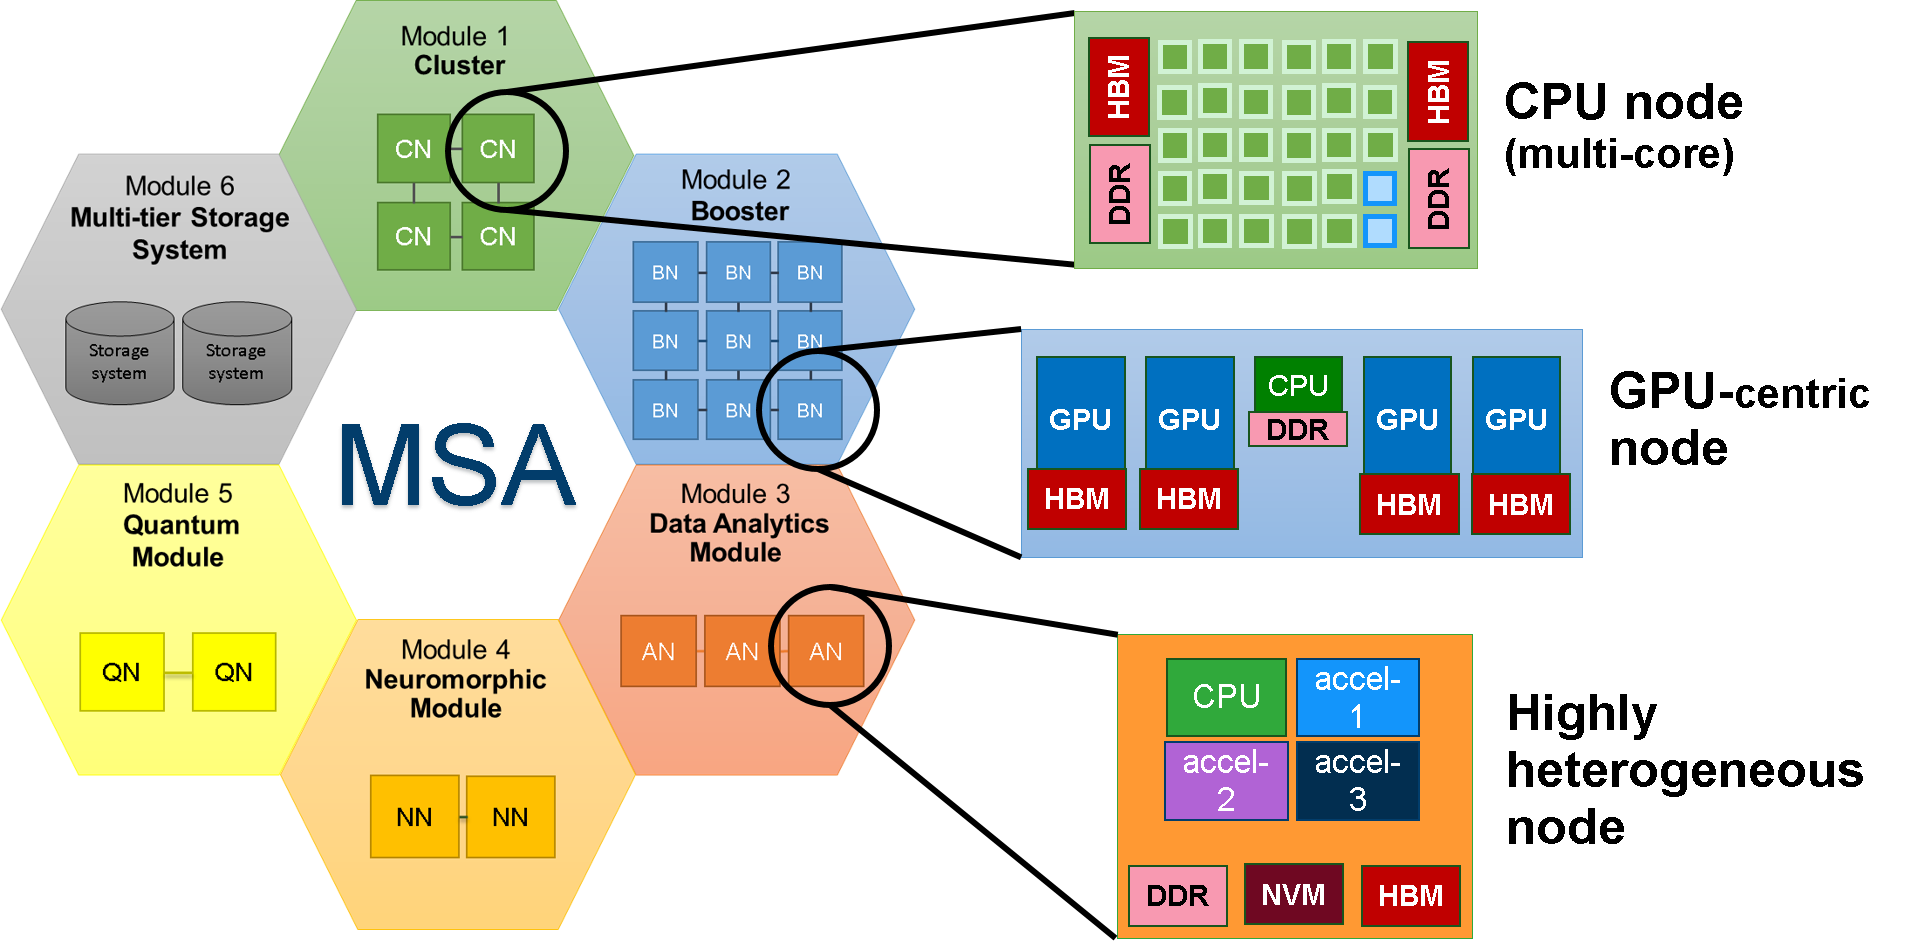
\includegraphics[width=0.9\linewidth]{images/modular_supercomputing_architecture.png}
\end{jsc}

\subsection{Speedup, Effizienz, Skalierbarkeit}

\begin{defi}{Speedup}
    % TODO: https://de.wikipedia.org/wiki/Speedup
    \emph{Speedup} beschreibt mathematisch den Zusammenhang zwischen der seriellen und der parallelen Ausführungszeit eines Programmteils.
    
    Der \emph{reale Speedup} $S$ einer parallelen Ausführung, der zur realen Messung herangezogen wird, kann wie folgt definiert werden:
    \[
        S = \frac{t_S}{t_p}
    \]
    Dabei sind $t_S$ und $t_p$ die serielle bzw. die parallele Ausführungszeit bei $p$ parallelen Bearbeitungseinheiten (Prozessoren).
\end{defi}

\begin{defi}{Amdahl's Law}
    % TODO: https://de.wikipedia.org/wiki/Speedup (Quelle)
    % TODO: https://de.wikipedia.org/wiki/Amdahlsches_Gesetz (Quelle)
    Das \emph{Amdahlsche Gesetz} (engl. \emph{Amdahl's Law}) ist ein Modell über die Beschleunigung von Programmen durch parallele Ausführung.
    Nach Amdahl wird der Geschwindigkeitszuwachs vor allem durch den sequentiellen Anteil des Problems beschränkt, da sich dessen Ausführungszeit durch Parallelisierung nicht verringern lässt.
    
    Der \emph{theoretische Speedup} $\eta_S$ nach Amdahl kann wie folgt definiert werden:
    \[
        \eta_S = \frac{t_S}{t_S \cdot f + t_S \cdot \frac{1-f}{p} } = \frac{t_S}{t_S \left((1 - f) + \frac{f}{n_P}\right)}
    \]
    Dabei sind $t_S$ und $t_p$ die serielle bzw. die parallele Ausführungszeit bei $p$ parallelen Bearbeitungseinheiten (Prozessoren);
    $f$ ist der Anteil der Laufzeit bzw. des Programms, der nicht parallel ablaufen kann und $n_P$ die Anzahl der Anzahl der Prozessoren, die zur Berechnung eingesetzt werden können.
    
    Es gelten weiterhin folgende Grenzwerte:
    \[
        \lim_{p \to \infty} \eta_S = \frac{1}{f} \quad \text{und} \quad \lim_{f \to 0 } \eta_S = n_P
    \]
\end{defi}

\begin{bonus}{Durchsatz}
    \emph{Durchsatz} ist ein Maß für die Bewertung der Verarbeitung einer gesamten Arbeitslast
    (mit welchem Flugzeug kann eine Fluggesellschaft mehr Personen befördern ?).
\end{bonus}

\begin{defi}{Effizienz}
    \emph{Effizienz} definiert das Verhältnis von Speedup und eingesetzter Prozessoranzahl.
    Sie drückt aus, welcher Anteil der Prozessorleistung nutzbar ist.
    
    Sie kann definiert werden als:
    \[
        E = \frac{S}{n_P} = \frac{t_S}{n_P\cdot t_P} \in (0; 1)
    \]
    \begin{align*}
        E(p) = \frac{S(p)}{p} =
        \frac{T(\text{sequentiell})}{p\cdot T(\text{parallel})},
        0<E(p)\leq 1
    \end{align*}
\end{defi}

\begin{example}[Speedup]{Skalarprodukt}
    Paralleler Algorithmus:
    \begin{enumerate}
        \item Aufteilen in $p$ Teilvektoren der Länge $\frac{n}{p}$
        \item jeder Prozessor berechnet das Skalarprodukt des Teilvektors $T_* (p) = \left(2 \cdot \frac{n}{p} - 1\right) \cdot t_\text{flop}$
        \item die Ergebnisse werden zu Prozessor 1 übertragen $T_t (p) = (p - 1) \cdot (t_\text{startup} + t_\text{word})$
        \item und Addition der Teilergebnisse (reduzieren) $T_+ (p) = (p - 1) \cdot t_\text{flop}$
    \end{enumerate}
    für $p=2^d$:
    \begin{align*}
        S(p) = \frac{T(\text{seq})}{T(p)} = \ldots =
        \frac{p}{\frac{p(\frac{2n}{p} + d-1)}{2n-1} + \frac{p\cdot d\cdot (t_\text{startup} + t_\text{word})}{(2n - 1)t_\text{flop}}}
    \end{align*}
    bei $n\gg p$:
    \begin{align*}
        \approx\frac{p}{
        \underbrace{1 + p\cdot \log_2 p}_{\text{Algorithmus}} \cdot
        \underbrace{\frac{1}{2n}}_{\text{Problemgröße}} \cdot
        \underbrace{\frac{t_\text{startup}}{t_\text{flop}}}_{\text{Hardware}}}
    \end{align*}
    
    TODO: Darstellung
\end{example}

\begin{example}[Effizienz]{Skalarprodukt}
    \[
        E(p) \approx \frac{1}{1 + n_P \cdot \log_2 n_P \cdot \frac{1}{2n} \cdot \frac{t_\text{startup}}{t_\text{flop}}}
    \]
    Die Effizienz
    \begin{itemize}
        \item \emph{steigt} mit wachsender Problemgröße $n$ (bei $n_P$ fest) und
        \item \emph{sinkt} bei größerer Prozessoranzahl $n_p$ (mit $n$ fest).
    \end{itemize}
    
    TODO: Darstellung\\
    TODO: Wie muss die Problemgröße $n$ wachsen bei festem $n_P$ und konstanter Effizienz?
\end{example}

\begin{defi}{Skalierbarkeit}
    Eine Rechnerarchitektur bzw. ein Programm ist \emph{skalierbar}, wenn die Effizienz der Programmbearbeitung bei wachsender Prozessorzahl gleich bleibt.
    Dies kann im Allgemeinen nur durch gleichzeitige Vergrößerung der Problemgröße erfolgen.
    
    Ein Programm bzw. ein Algorithmus ist \emph{perfekt skalierbar}, wenn $n \in \mathcal{O}(n_P)$ ist, also linear in $n_P$.
    
    TODO: Was soll das heißen?
\end{defi}

\begin{defi}{Paralleler Overhead}
    
    Der Speedup kann sich reduzieren durch zusätzlichen \emph{parallelen Overhead}.
    
    \[
        V(n_P) = n_P \cdot t_P - t_S
    \]
    
    Der \emph{durchschnittliche parallele Overhead} ist definiert als:
    \[
        \overline{V}(n_P) = \frac{V(n_P)}{n_P}
    \]
    
    Er wird verursacht durch:
    \begin{itemize}
        \item Kosten für das Starten eines Vorgangs (\enquote{startup}),
        \item Kosten für das Verteilen bzw. Verwalten gemeinsamer Daten, oder
        \item Kosten für Synchronisation.
    \end{itemize}
    
    Daher gilt abzuwägen zwischen:
    \begin{itemize}
        \item Verkleinern der Kommunikation durch größere Arbeitspakete (\emph{grobkörnige Granualität})
        \item Kleine Arbeitspaketen, damit viele Prozessoren arbeiten (\emph{feinkörnige Granualität})
    \end{itemize}
    
    TODO: Sinnvolle Definition finden
\end{defi}

\subsection{Aufgaben}

\begin{aufgabe}{Speedup}
    Ein sequentielles Programm lasse sich zu $80\%$ parallelisieren. 
    Welcher Speedup kann mit 20 Prozessoren erzielt werden?
    \tcblower
    Der Speedup ist definiert durch: 
    \begin{align*}
        \eta_S = \frac{t_S}{t_S \cdot f + t_S \cdot \frac{1-f}{p}}
    \end{align*}
    mit $t_S=1$, $f=1-0.8=0.2$, $p=20$ ist der Speedup eines Programmes dann:
    \begin{align*}
        \eta_S = \frac{1}{1 \cdot 0.2 + 1 \cdot \frac{0.8}{20}} = \frac{25}{6} \approx 4.1667
    \end{align*}
\end{aufgabe}

\begin{aufgabe}{Skalierbarkeit}
    Wann ist eine Rechnerarchitektur bzw. ein Programm skalierbar?
    \tcblower
    Wenn die Effizienz der Programmbearbeitung bei wachsender Prozessorzahl gleich bleibt.
\end{aufgabe}

\begin{aufgabe}{Pipelining}
    Wie berechnet sich der Speedup $\eta_S$ bei Pipeline-Nutzung mit n Aufträgen und k Stufen?
    \tcblower
    Der Speedup berechnet sich durch: 
    \begin{align*}
        \eta_S = \frac{n\cdot k}{n+k-1}
    \end{align*}
\end{aufgabe}
